\documentclass[12pt]{mwart}
\usepackage{polski}
\usepackage[utf8]{inputenc}
\usepackage[T1]{fontenc}
\usepackage{lmodern}
\usepackage{mathtools,amsthm,amssymb,icomma,upgreek,xfrac,enumitem,multicol,paracol,amsmath}
%\usepackage[hidelinks,breaklinks,pdfusetitle,pdfdisplaydoctitle]{hyperref}
\usepackage{cancel}
\mathtoolsset{showonlyrefs,mathic}
\title{\textbf{Raport 1.}}
\author{\fontsize{12pt}{12pt}\selectfont \emph{Klaudia Janicka, 262268}}
\date{10 maja 2022}
\usepackage{float,hyperref}
\usepackage{extsizes}
\usepackage[margin=0.3in]{geometry}

%\setlist[enumerate]{}
\setlist[itemize]{itemsep=0.3em}

\DeclareMathOperator{\diff}{d\!}

\begin{document}
	\maketitle
	\section{Informacje}
	\noindent Dane pochodzą ze strony finance.yahoo.com. Zbiory danych to odpowiednio: X - kurs funta brytyjskiego w przeliczeniu na dolary (GBP/USD), Y - kurs euro w przeliczeniu na dolary (EUR/USD). Do analizy użyto dziennych danych z okresu 5 lat, od 17 kwietnia 2017 roku do 17 kwietnia 2022 roku. Ze zbiorów zostały usunięte wiersze z brakiem danych. Ostateczna liczba wierszy obu zbiorów wynosi 1303.
	\section{Analiza}
	\begin{table}[H]
		\centering
		\begin{tabular}{|l|l|l|} 
			\hline
			\phantom{a} & $X$&$Y$ \\ \hline
			\text{Mediana} & 1.3120 & 1.1532 \\ \hline
			\text{Kwartyl rzędu $\frac{1}{4}$} & 1.2866 & 1.1207 \\ \hline
			\text{Kwartyl rzędu $\frac{3}{4}$} & 1.3558 & 1.1842 \\ \hline
			\text{Rozstęp międzykwartylowy} & 0.0691 & 0.0635 \\ \hline
			\text{Rozstęp} & 0.2845  &0.1901 \\ \hline
			\text{Wariancja} & 0.0026 &0.0017 \\ \hline
			\text{Odchylenie standardowe} & 0.0507&0.0415 \\ \hline
			\text{Współczynnik zmienności} & 3.8500 & 3.6000 \\ \hline
		\end{tabular}
	\end{table}
	%scaterplot
	\begin{figure}[H]
		\begin{minipage}{.5\linewidth}
			\centering
			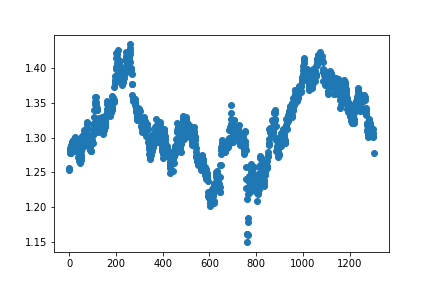
\includegraphics[scale=0.7]{X_sc.PNG}
			\caption{Scatterplot zbioru X}
		\end{minipage}
		$\quad$
		\begin{minipage}{.5\linewidth}
			\centering
			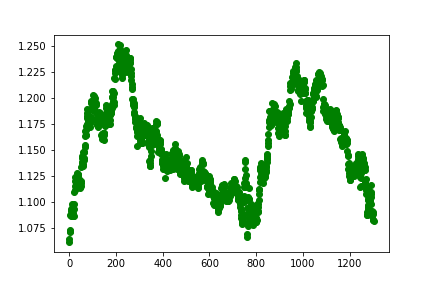
\includegraphics[scale=0.7]{Y_sc.PNG}
			\caption{Scatterplot zbioru Y}
		\end{minipage}
	\end{figure}
	\section{Interpretacja}
	\begin{table}[H]
		\centering
		\begin{tabular}{|l|l|l|} 
			\hline
			\text{Średnia} & $X$&$Y$ \\ \hline
			\text{Arytmetyczna} & 1.3177 & 1.1541 \\ \hline
			\text{Geometryczna} & 1.3167 & 1.1537 \\ \hline
			\text{Harmoniczna} & 1.3157  &1.1526 \\ \hline
		\end{tabular}
	\end{table}
%Hist
\begin{figure}[H]
	\begin{minipage}{.5\linewidth}
		\centering
		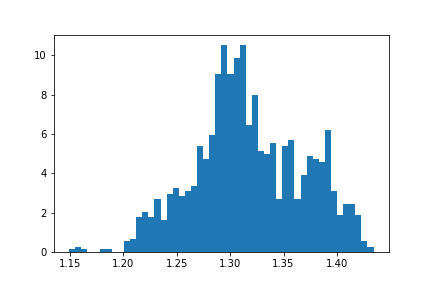
\includegraphics[scale=0.7]{X_hist.PNG}
		\caption{Histogram zbioru X}
	\end{minipage}
	$\quad$
	\begin{minipage}{.5\linewidth}
		\centering
		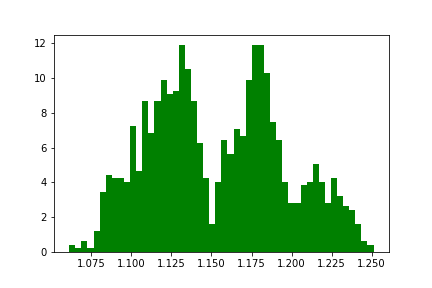
\includegraphics[scale=0.7]{Y_hist.PNG}
		\caption{Histogram zbioru Y}
	\end{minipage}
\end{figure}
%Gęstość
\begin{figure}[H]
	\begin{minipage}{.5\linewidth}
		\centering
		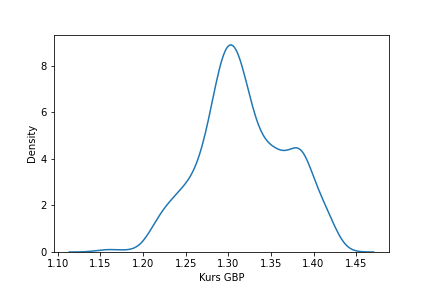
\includegraphics[scale=0.7]{X_kde.PNG}
		\caption{Gęstość zbioru X}
	\end{minipage}
	$\quad$
	\begin{minipage}{.5\linewidth}
		\centering
		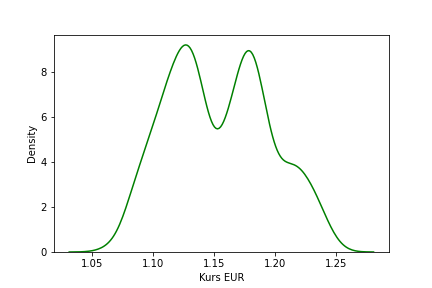
\includegraphics[scale=0.7]{Y_kde.PNG}
		\caption{Gęstość zbioru Y}
	\end{minipage}
\end{figure}
%Dystrybuanta
\begin{figure}[H]
	\begin{minipage}{.5\linewidth}
		\centering
		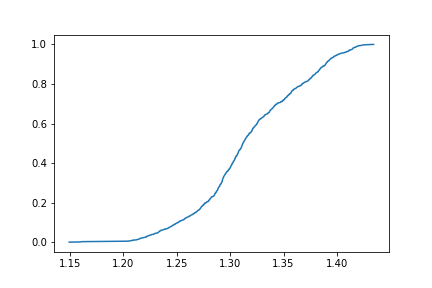
\includegraphics[scale=0.7]{X_cdf.PNG}
		\caption{Dystrybuanta zbioru X}
	\end{minipage}
	$\quad$
	\begin{minipage}{.5\linewidth}
		\centering
		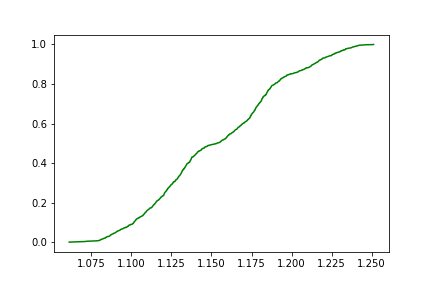
\includegraphics[scale=0.7]{Y_cdf.PNG}
		\caption{Dystrybuanta zbioru Y}
	\end{minipage}
\end{figure}
%Średnie ucinane
\begin{figure}[H]
	\begin{minipage}{.5\linewidth}
		\centering
		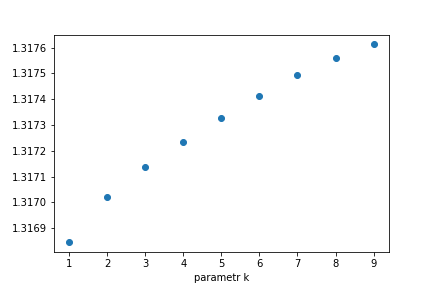
\includegraphics[scale=0.7]{X_trim.PNG}
		\caption{Średnia ucinana zbioru X}
	\end{minipage}
	$\quad$
	\begin{minipage}{.5\linewidth}
		\centering
		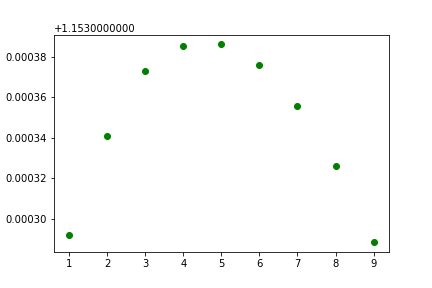
\includegraphics[scale=0.7]{Y_trim.PNG}
		\caption{Średnia ucinana zbioru Y}
	\end{minipage}
\end{figure}
%średnie winsorowskie
\begin{figure}[H]
	\begin{minipage}{.5\linewidth}
		\centering
		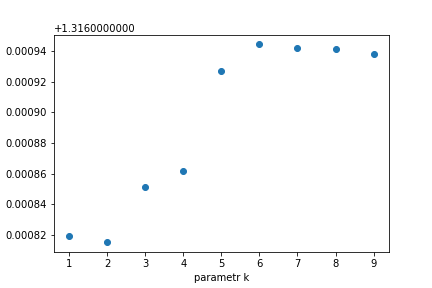
\includegraphics[scale=0.7]{X_wins.PNG}
		\caption{Średnia winsorowska zbioru X}
	\end{minipage}
	$\quad$
	\begin{minipage}{.5\linewidth}
		\centering
		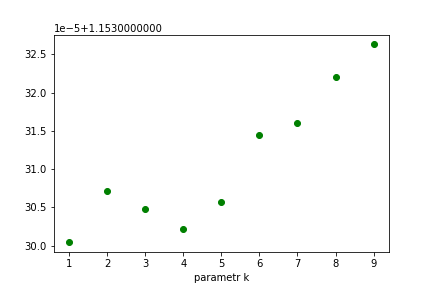
\includegraphics[scale=0.7]{Y_wins.PNG}
		\caption{Średnia winsorowska zbioru Y}
	\end{minipage}
\end{figure}
	\section{Porównanie}
	\noindent Korelacja zbiorów jest dość wysoka i wynosi $\sim 0.77$. Oznacza to, że, gdy wzrasta jedna z wartości, druga też wzrasta i odwrotnie.
	%gęstość porównanie
	\begin{figure}[H]
			\centering
			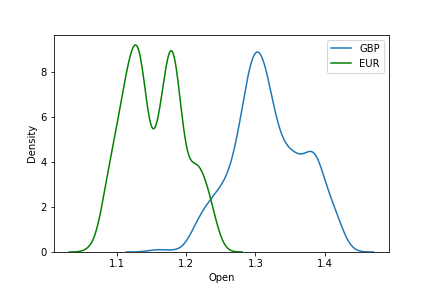
\includegraphics[scale=0.7]{XY_kde.PNG}
			\caption{Porównanie gęstości zbiorów X i Y}
	\end{figure}
	%boxplot
	\begin{figure}[H]
		\begin{minipage}{.5\linewidth}
			\centering
			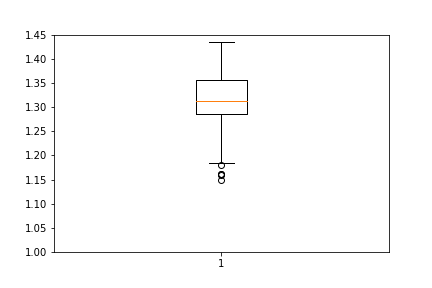
\includegraphics[scale=0.7]{X_box.PNG}
			\caption{Boxplot zbioru X}
		\end{minipage}
		$\quad$
		\begin{minipage}{.5\linewidth}
			\centering
			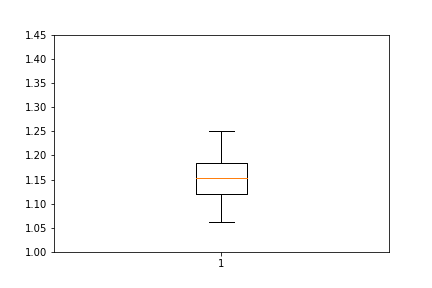
\includegraphics[scale=0.7]{Y_box.PNG}
			\caption{Boxplot zbioru Y}
		\end{minipage}
	\end{figure}
\noindent Widzimy, że zbiór X ma co najmniej 3 wartości odstające, podczas gdy Y nie ma żadnej. Mediana zbioru X jest przesunięta w stronę pierwszego kwartyla, zbioru Y wydaje się być na dokładnie pomiędzy kwartylami. Najniższa wartość X jest mocniej wysunięta niż najwyższa, podczas gdy Y są rozmieszczone w podobnej odległości od kwartyli. Żaden ze zbiorów nie ma górnej ani dolnej obserwacji ekstremalnej.
	\section{Podsumowanie}
\end{document}